% Options for packages loaded elsewhere
\PassOptionsToPackage{unicode}{hyperref}
\PassOptionsToPackage{hyphens}{url}
\PassOptionsToPackage{dvipsnames,svgnames,x11names}{xcolor}
%
\documentclass[
  letterpaper,
  DIV=11,
  numbers=noendperiod]{scrartcl}

\usepackage{amsmath,amssymb}
\usepackage{iftex}
\ifPDFTeX
  \usepackage[T1]{fontenc}
  \usepackage[utf8]{inputenc}
  \usepackage{textcomp} % provide euro and other symbols
\else % if luatex or xetex
  \usepackage{unicode-math}
  \defaultfontfeatures{Scale=MatchLowercase}
  \defaultfontfeatures[\rmfamily]{Ligatures=TeX,Scale=1}
\fi
\usepackage{lmodern}
\ifPDFTeX\else  
    % xetex/luatex font selection
    \setmainfont[]{Roboto-Regular.ttf}
\fi
% Use upquote if available, for straight quotes in verbatim environments
\IfFileExists{upquote.sty}{\usepackage{upquote}}{}
\IfFileExists{microtype.sty}{% use microtype if available
  \usepackage[]{microtype}
  \UseMicrotypeSet[protrusion]{basicmath} % disable protrusion for tt fonts
}{}
\makeatletter
\@ifundefined{KOMAClassName}{% if non-KOMA class
  \IfFileExists{parskip.sty}{%
    \usepackage{parskip}
  }{% else
    \setlength{\parindent}{0pt}
    \setlength{\parskip}{6pt plus 2pt minus 1pt}}
}{% if KOMA class
  \KOMAoptions{parskip=half}}
\makeatother
\usepackage{xcolor}
\setlength{\emergencystretch}{3em} % prevent overfull lines
\setcounter{secnumdepth}{-\maxdimen} % remove section numbering
% Make \paragraph and \subparagraph free-standing
\makeatletter
\ifx\paragraph\undefined\else
  \let\oldparagraph\paragraph
  \renewcommand{\paragraph}{
    \@ifstar
      \xxxParagraphStar
      \xxxParagraphNoStar
  }
  \newcommand{\xxxParagraphStar}[1]{\oldparagraph*{#1}\mbox{}}
  \newcommand{\xxxParagraphNoStar}[1]{\oldparagraph{#1}\mbox{}}
\fi
\ifx\subparagraph\undefined\else
  \let\oldsubparagraph\subparagraph
  \renewcommand{\subparagraph}{
    \@ifstar
      \xxxSubParagraphStar
      \xxxSubParagraphNoStar
  }
  \newcommand{\xxxSubParagraphStar}[1]{\oldsubparagraph*{#1}\mbox{}}
  \newcommand{\xxxSubParagraphNoStar}[1]{\oldsubparagraph{#1}\mbox{}}
\fi
\makeatother


\providecommand{\tightlist}{%
  \setlength{\itemsep}{0pt}\setlength{\parskip}{0pt}}\usepackage{longtable,booktabs,array}
\usepackage{calc} % for calculating minipage widths
% Correct order of tables after \paragraph or \subparagraph
\usepackage{etoolbox}
\makeatletter
\patchcmd\longtable{\par}{\if@noskipsec\mbox{}\fi\par}{}{}
\makeatother
% Allow footnotes in longtable head/foot
\IfFileExists{footnotehyper.sty}{\usepackage{footnotehyper}}{\usepackage{footnote}}
\makesavenoteenv{longtable}
\usepackage{graphicx}
\makeatletter
\def\maxwidth{\ifdim\Gin@nat@width>\linewidth\linewidth\else\Gin@nat@width\fi}
\def\maxheight{\ifdim\Gin@nat@height>\textheight\textheight\else\Gin@nat@height\fi}
\makeatother
% Scale images if necessary, so that they will not overflow the page
% margins by default, and it is still possible to overwrite the defaults
% using explicit options in \includegraphics[width, height, ...]{}
\setkeys{Gin}{width=\maxwidth,height=\maxheight,keepaspectratio}
% Set default figure placement to htbp
\makeatletter
\def\fps@figure{htbp}
\makeatother

\newfontfamily\sectionfont{PixelOperatorSC.ttf}
\newfontfamily\subsectionfont{PixelOperatorSC.ttf}
\newfontfamily\subsubsectionfont{PixelOperatorSC.ttf}
\addtokomafont{section}{\sectionfont}
\addtokomafont{subsection}{\subsectionfont}
\addtokomafont{subsubsection}{\subsubsectionfont}
\usepackage{fontspec}
\usepackage{fancyhdr}
\usepackage{graphicx}
\usepackage{textpos}
\usepackage{background}
\usepackage[french]{babel}
\usepackage{datetime2}
\DTMsetdatestyle{french}
\pagestyle{fancy}
\usepackage[a4paper,margin=1.87cm,includefoot]{geometry}
\renewcommand{\headrulewidth}{0pt}
\newfontfamily\headerfont{PixelOperatorSC.ttf}
\fancyhead[L]{\headerfont CAPP/CLESSN}
\fancyhead[C]{\headerfont Rapport présenté à Léger}
\fancyhead[R]{\headerfont Datagotchi Canada 2025}
\fancyfoot[C]{\vspace*{0.5cm}\thepage}
\KOMAoption{captions}{tableheading}
\makeatletter
\@ifpackageloaded{caption}{}{\usepackage{caption}}
\AtBeginDocument{%
\ifdefined\contentsname
  \renewcommand*\contentsname{Table of contents}
\else
  \newcommand\contentsname{Table of contents}
\fi
\ifdefined\listfigurename
  \renewcommand*\listfigurename{List of Figures}
\else
  \newcommand\listfigurename{List of Figures}
\fi
\ifdefined\listtablename
  \renewcommand*\listtablename{List of Tables}
\else
  \newcommand\listtablename{List of Tables}
\fi
\ifdefined\figurename
  \renewcommand*\figurename{Figure}
\else
  \newcommand\figurename{Figure}
\fi
\ifdefined\tablename
  \renewcommand*\tablename{Table}
\else
  \newcommand\tablename{Table}
\fi
}
\@ifpackageloaded{float}{}{\usepackage{float}}
\floatstyle{ruled}
\@ifundefined{c@chapter}{\newfloat{codelisting}{h}{lop}}{\newfloat{codelisting}{h}{lop}[chapter]}
\floatname{codelisting}{Listing}
\newcommand*\listoflistings{\listof{codelisting}{List of Listings}}
\makeatother
\makeatletter
\makeatother
\makeatletter
\@ifpackageloaded{caption}{}{\usepackage{caption}}
\@ifpackageloaded{subcaption}{}{\usepackage{subcaption}}
\makeatother

\ifLuaTeX
  \usepackage{selnolig}  % disable illegal ligatures
\fi
\usepackage{bookmark}

\IfFileExists{xurl.sty}{\usepackage{xurl}}{} % add URL line breaks if available
\urlstyle{same} % disable monospaced font for URLs
\hypersetup{
  colorlinks=true,
  linkcolor={blue},
  filecolor={Maroon},
  citecolor={Blue},
  urlcolor={Blue},
  pdfcreator={LaTeX via pandoc}}


\author{}
\date{}

\begin{document}


\begin{titlepage}
  \newfontfamily\titlepagefont{PixelOperatorSC.ttf}

  % Background image setup
  \backgroundsetup{
    scale=1.3,
    color=black,
    opacity=0.5,
    angle=0,
    position=current page.south,
    vshift=2.2cm,
    hshift=0cm,
    contents={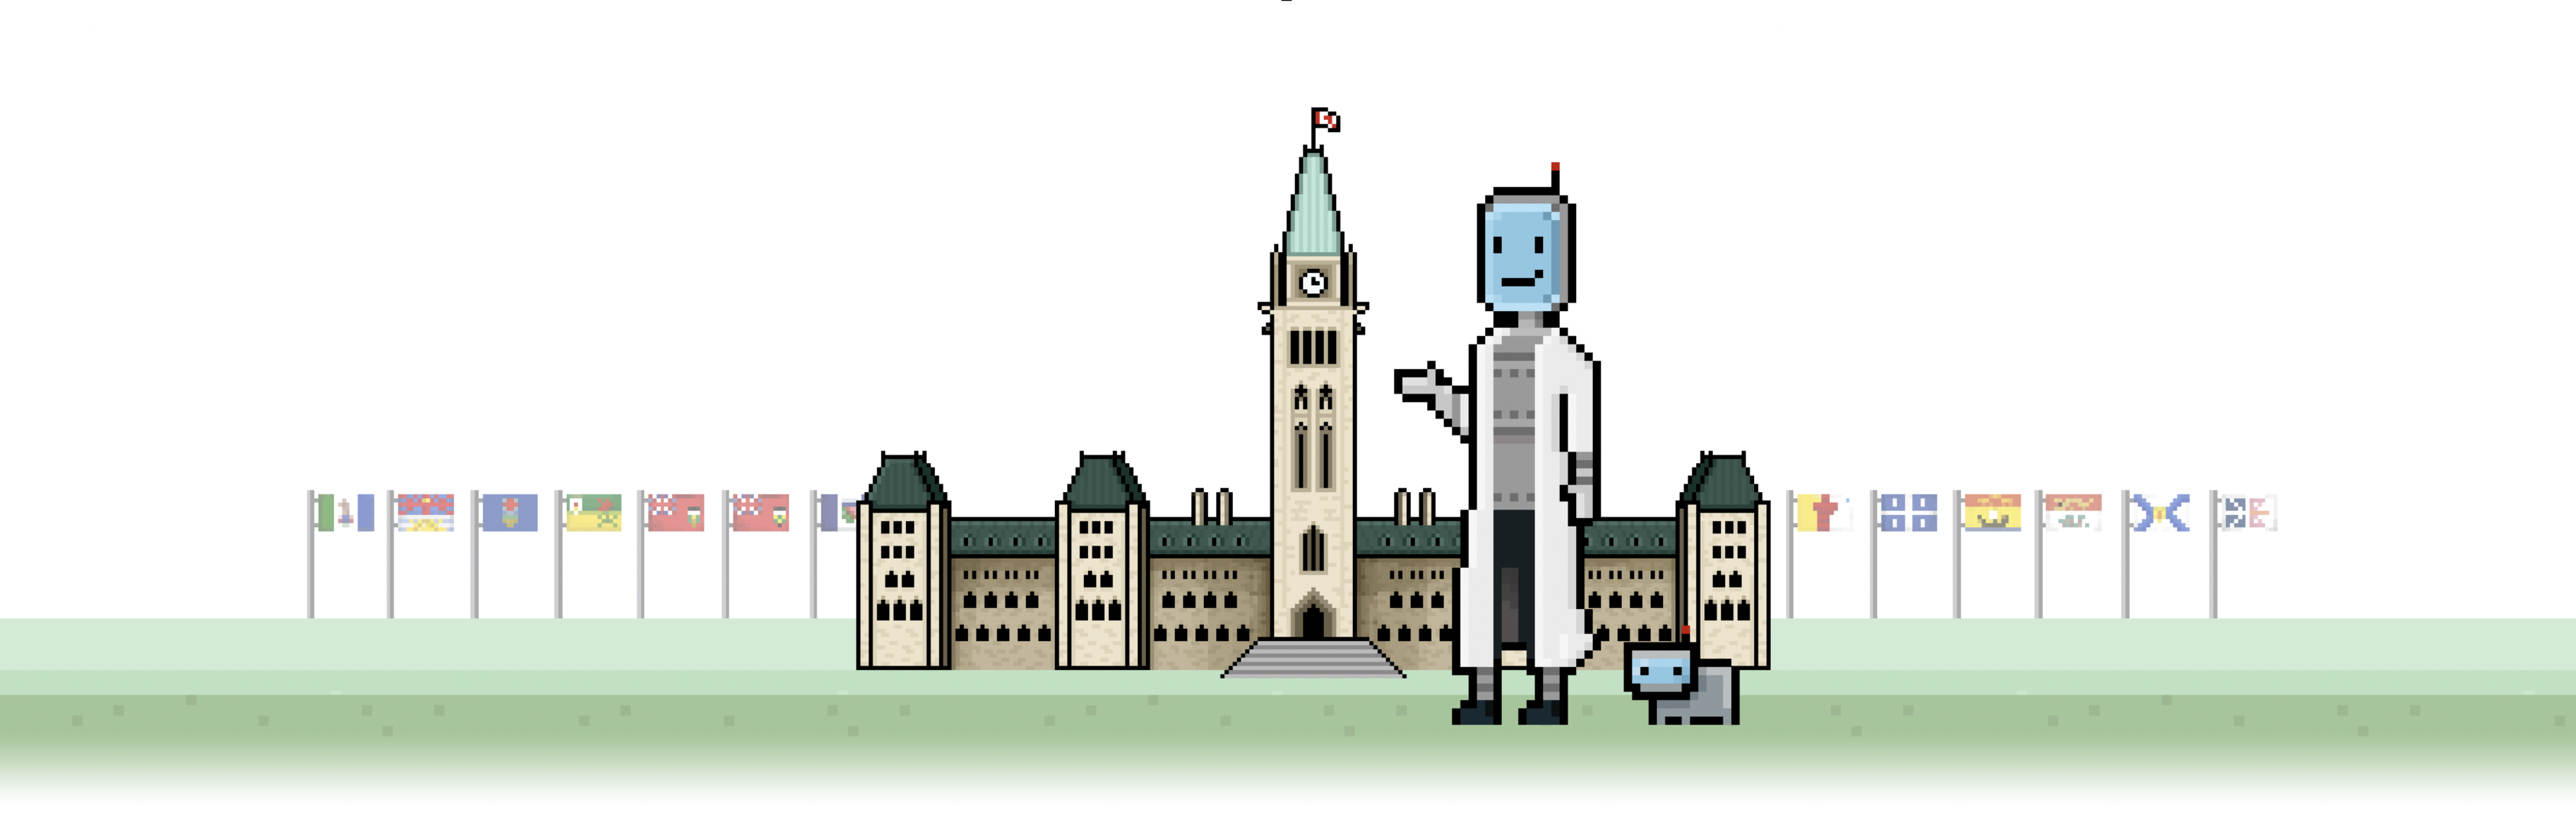
\includegraphics[width=1\textwidth]{img/datagotchi_canada.png}}
  }

  \begin{center}
    \null\vspace{\stretch{1}} % Ensures vertical centering
    {\titlepagefont\fontsize{48pt}{18pt}\selectfont \textbf{Léger-Datagotchi}}\\[1cm]
    {\titlepagefont\fontsize{25pt}{18pt}\selectfont \textbf{Report on Coffee-Transport Dynamics}}\\[1cm]
    
\includegraphics[width=0.2\textwidth]{img/leger_small.png}\\[4cm]
    {\titlepagefont\fontsize{16pt}{16pt}\selectfont \textbf{Center for Public Policy Analysis (CAPP)}}\\[0.5cm]
    {\titlepagefont\fontsize{16pt}{16pt}\selectfont \textbf{Leadership Chair in the Teaching of Digital Social Science (CLESSN)}}\\[3cm]
    {\titlepagefont\fontsize{16pt}{16pt}\selectfont \textbf{Université Laval}}\\[0.5cm]
    {\titlepagefont\fontsize{16pt}{16pt}\selectfont \textbf{Université de Montréal}}\\[1cm]
    {\titlepagefont\fontsize{12pt}{12pt}\selectfont \copyright \thinspace CLESSN, March 25, 2025}\\
    \null\vspace{\stretch{2}} % Ensures vertical centering
  \end{center}  \thispagestyle{empty} % Prevents headers and footers on the title page
  \clearpage % Ensures the next content starts on a clean page
\end{titlepage}
\backgroundsetup{contents={}}

\setcounter{page}{1}

\section{The Coffee Battle in Canada}\label{the-coffee-battle-in-canada}

The map illustrates the regional dominance of coffee chains across
Canada, revealing a significant geographic divide. Tim Hortons largely
dominates in rural regions and in the eastern part of the country,
affirming its status as a national symbol with more than 60\% of
electoral districts under its influence. Conversely, Starbucks is mainly
established in major urban centers such as Vancouver and certain parts
of Toronto, demonstrating an urban-rural divide in consumer preferences.
McDonald's, on the other hand, finds its strongholds in intermediate
zones and certain suburbs, reflecting a positioning strategy between the
two other giants.

\begin{figure}[H]

{\centering \includegraphics[width=0.8\textwidth,height=\textheight]{_SharedFolder_datagotchi_federal_2024/graph/analyses/café/bataille_cafe_canada_light_avec_logo-EN.png}

}

\caption{The Coffee Battle in Canada}

\end{figure}%

\section{The Coffee-Politics Index}\label{the-coffee-politics-index}

The coffee-politics index graph reveals a fascinating correlation
between partisan preferences and coffee consumption habits. Conservative
voters display a marked affinity for Tim Hortons (+8.2 points above the
national average), illustrating the symbolic attachment to traditional
Canadian values that this chain represents. In contrast, supporters of
progressive parties such as the NDP and the Green Party show a
significant preference for Starbucks (respectively +4.6 and +5.9
points), a chain associated with a more cosmopolitan image. The Bloc
Québécois presents a distinct profile with above-average McDonald's
consumption, which could reflect Quebec's cultural particularities. This
distribution reveals how everyday consumption choices surprisingly align
with political values, transforming coffee into a marker of social
identity in Canada.

\begin{figure}[H]

{\centering 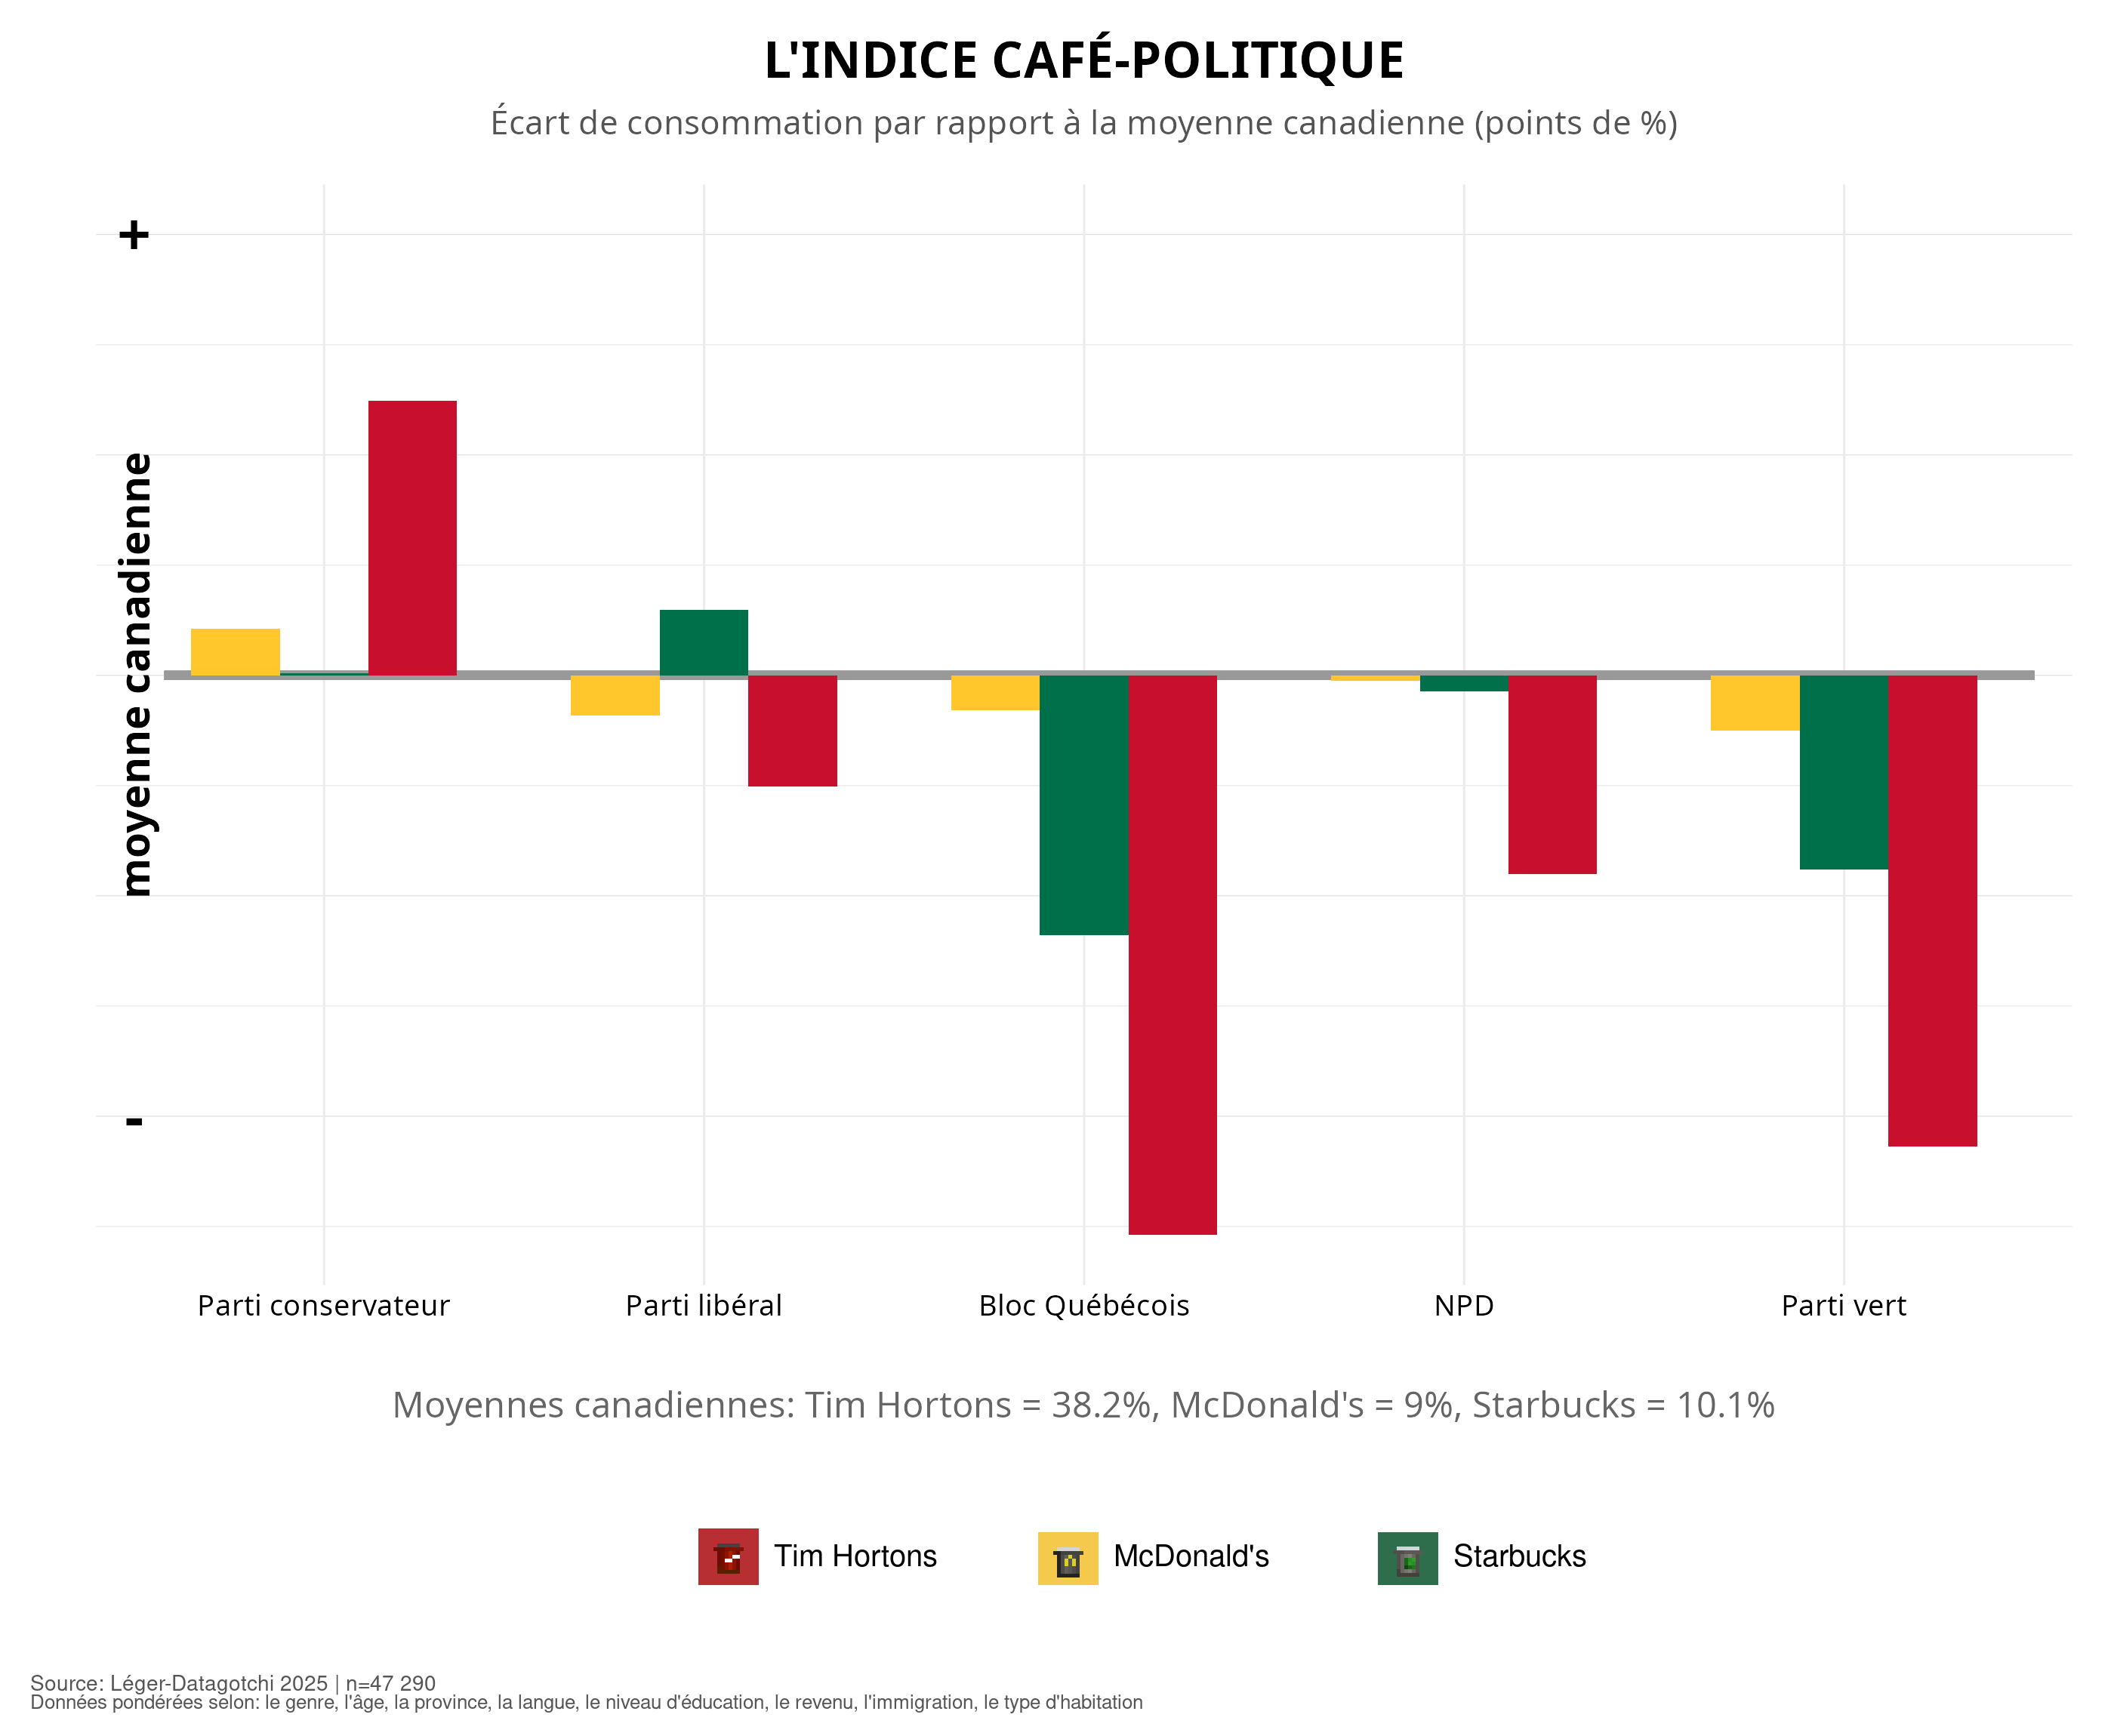
\includegraphics[width=1\textwidth,height=\textheight]{img/cafe_graph.png}

}

\caption{Coffee-Politics Index}

\end{figure}%%
\begin{figure}[H]

{\centering \includegraphics[width=0.9\textwidth,height=\textheight]{_SharedFolder_datagotchi_federal_2024/graph/analyses/café/coffee_politics_triple-FR.png}

}

\caption{Coffee-Politics Index (Triple Analysis)}

\end{figure}%

The graph presents coffee consumption by political affiliation across
three different chains, with distinct vertical scales for each chain.
For Tim Hortons (scale from 0\% to 50\%), CPC supporters are the largest
consumers (about 44\%), followed by the LPC (about 36\%), the NDP (about
33\%), the Green Party (about 27\%), and finally the BQ which shows the
lowest consumption (about 25\%). For McDonald's (scale from 0\% to
20\%), the distribution is more uniform across parties. The CPC comes
slightly ahead (about 10\%), followed by the NDP (about 7-8\%), then the
BQ and the LPC at similar levels (about 6-7\%), and finally the Green
Party (about 5-6\%). For Starbucks (scale from 0\% to 10\%), the LPC
clearly dominates (about 38\%), followed by the NDP (about 32\%), the
CPC (about 30\%), the Green Party (about 19\%), and finally the BQ which
shows the lowest consumption (about 14\%).

\section{The Transport Battle in
Canada}\label{the-transport-battle-in-canada}

This map illustrates the regional dominance of transportation modes
across Canada, revealing a significant geographic divide. Cars
predominantly dominate in rural regions and in the eastern part of the
country, affirming their status as the primary means of transportation
with the majority of electoral districts under their influence,
represented in blue on the map. Conversely, public transportation is
mainly established in major urban centers such as Toronto and certain
parts of Montreal and Vancouver, demonstrating an urban-rural divide in
travel preferences. Motorcycles, meanwhile, find their strongholds in
the northern part of the country, particularly in territories such as
Nunavut and the Northwest Territories, perhaps reflecting specific
regional preferences or geographic constraints. There are also some
areas where walking (in yellow) is the dominant mode, particularly
visible in certain parts of Vancouver and Manitoba, while SUVs (in red)
are preferred in certain regions of Quebec, notably in western Montreal.

\begin{figure}[H]

{\centering 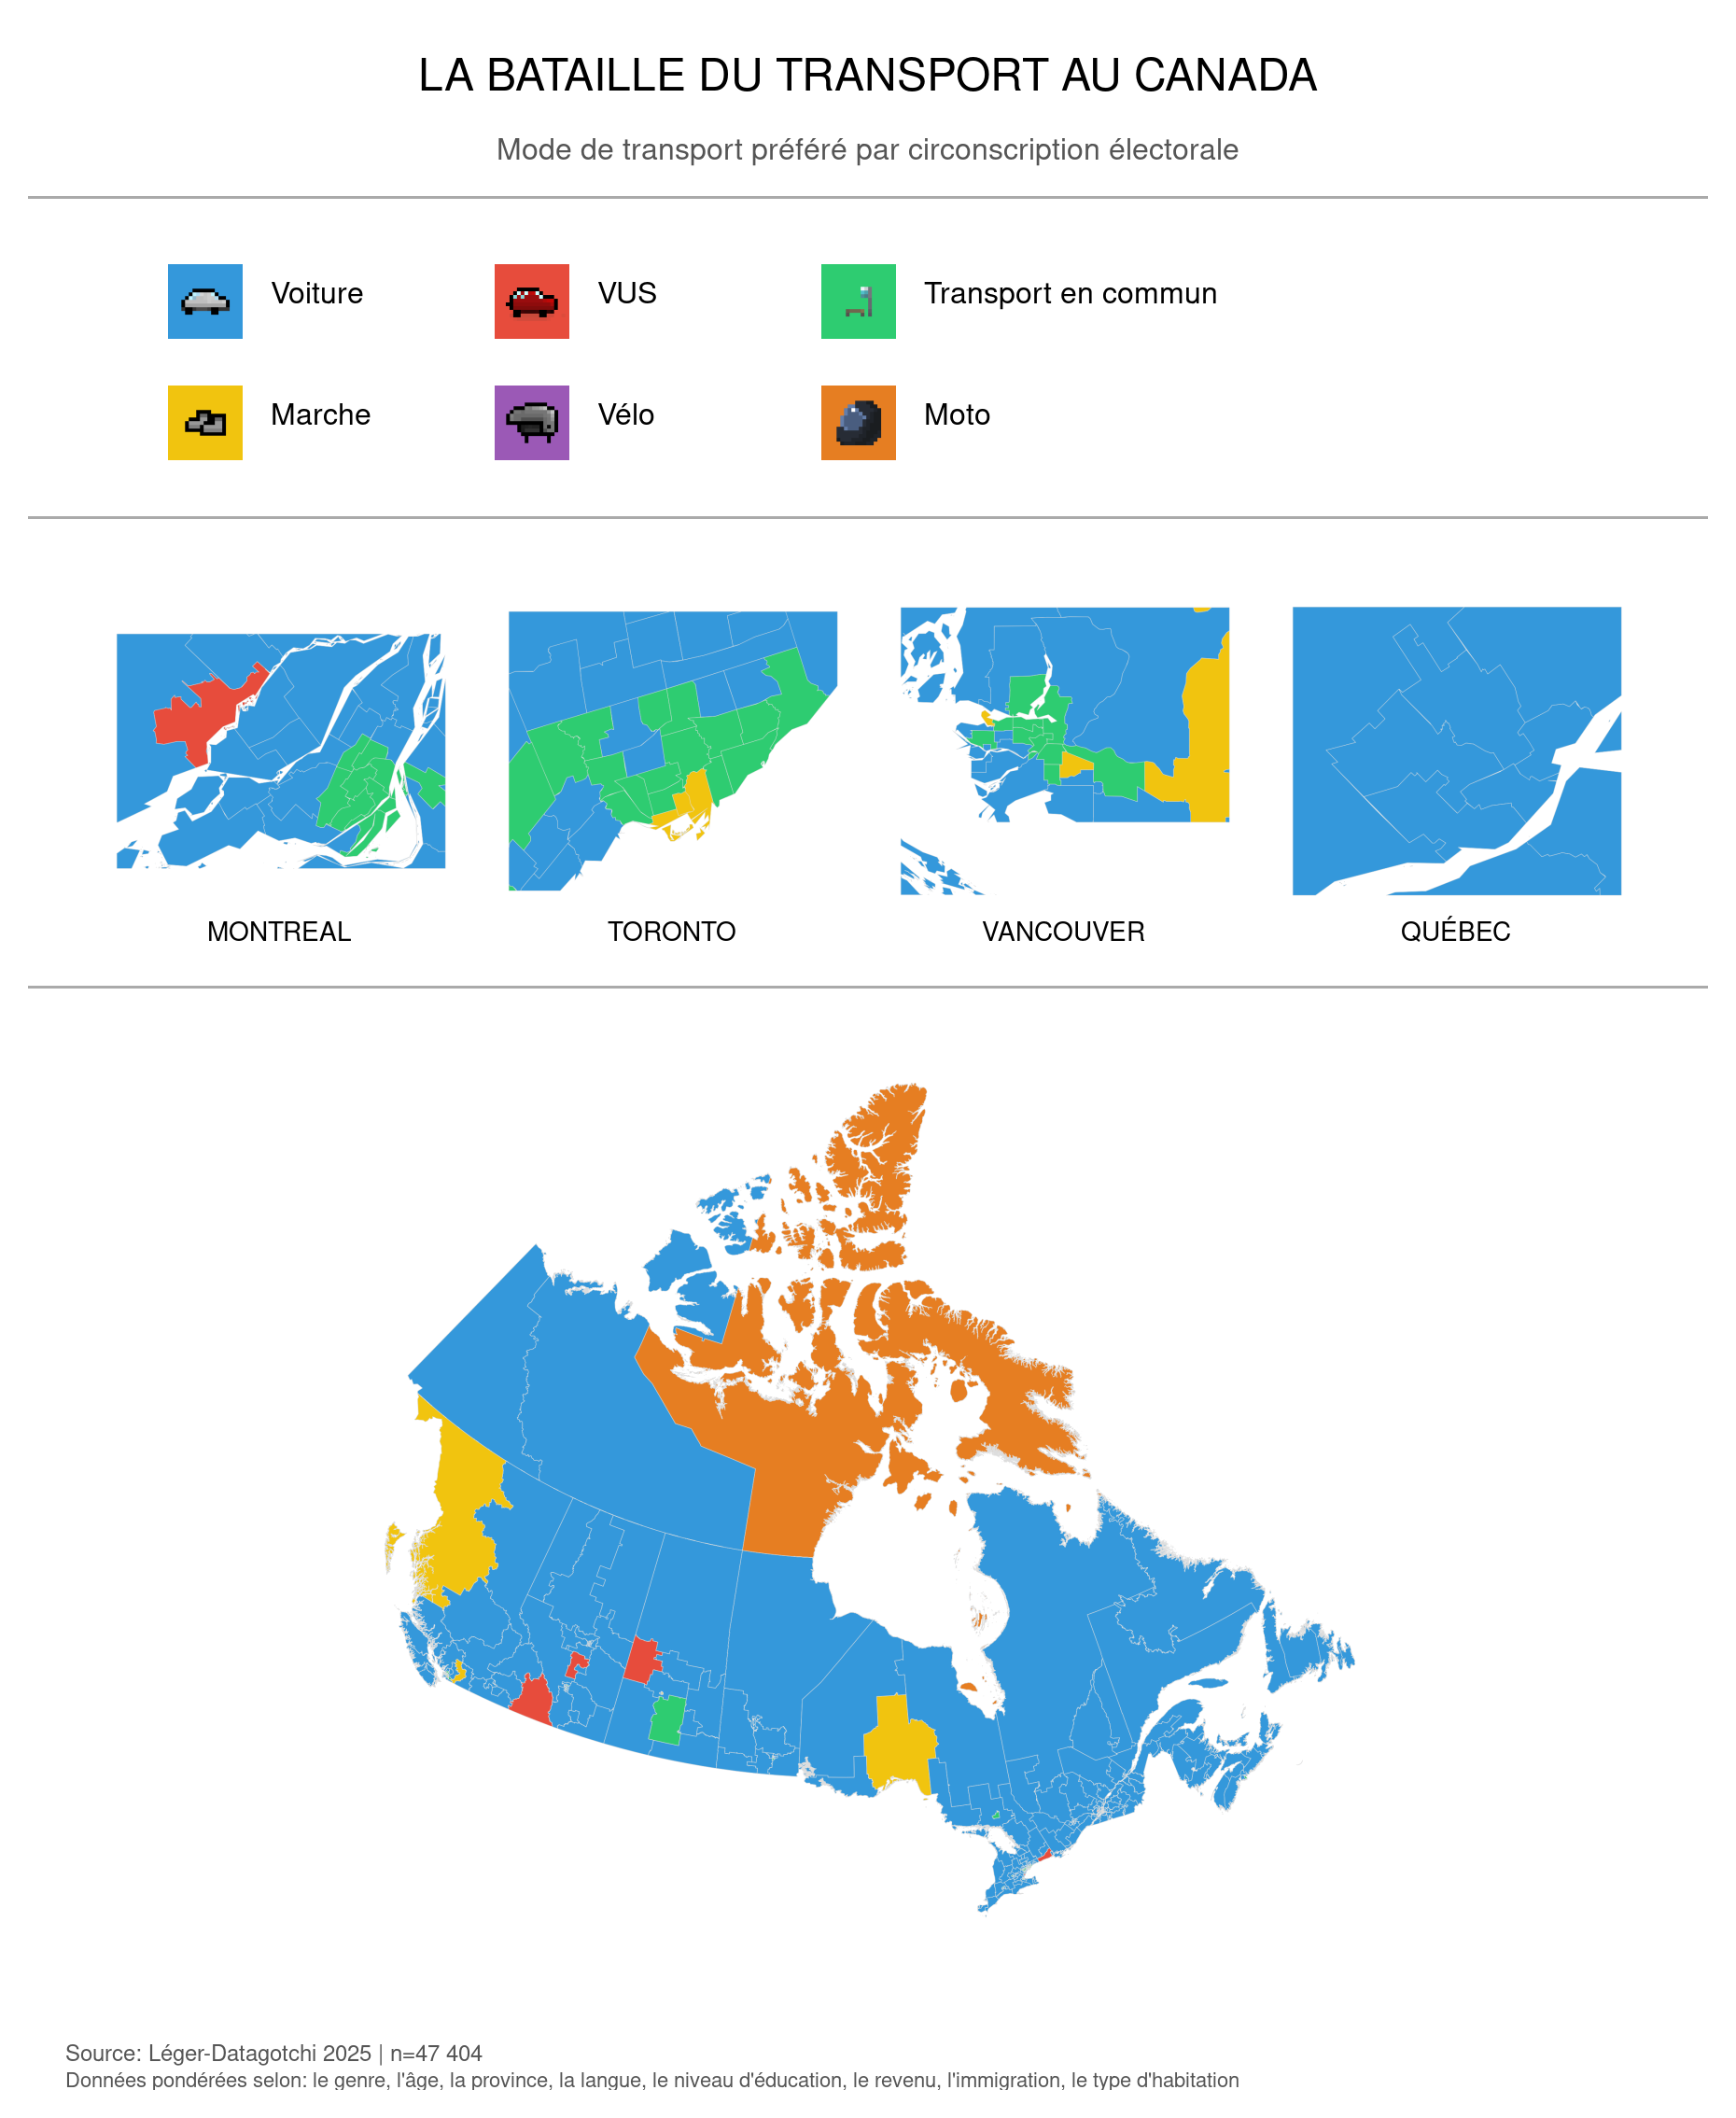
\includegraphics[width=0.75\textwidth,height=\textheight]{img/transport_map.png}

}

\caption{The Transport Battle in Canada}

\end{figure}%

\section{The Transport-Politics
Index}\label{the-transport-politics-index}

This graph illustrates the relationship between transportation
preferences and political affiliations in Canada, revealing significant
ideological divides. The Conservative Party seems to show an
overrepresentation of car drivers compared to the national average,
while underrepresenting public transportation users and pedestrians.
Conversely, the Bloc Québécois seems to present a deficit of public
transportation users, offset by a slight overrepresentation of car and
SUV drivers, perhaps reflecting the specific geographic realities of
Quebec. The NDP and the Green Party, meanwhile, seem to attract more
pedestrians and cyclists, with an underrepresentation of car drivers in
the NDP. The national average indicates that cars remain dominant
(47\%), followed by public transportation (24.8\%) and walking (13.8\%).

\begin{figure}[H]

{\centering 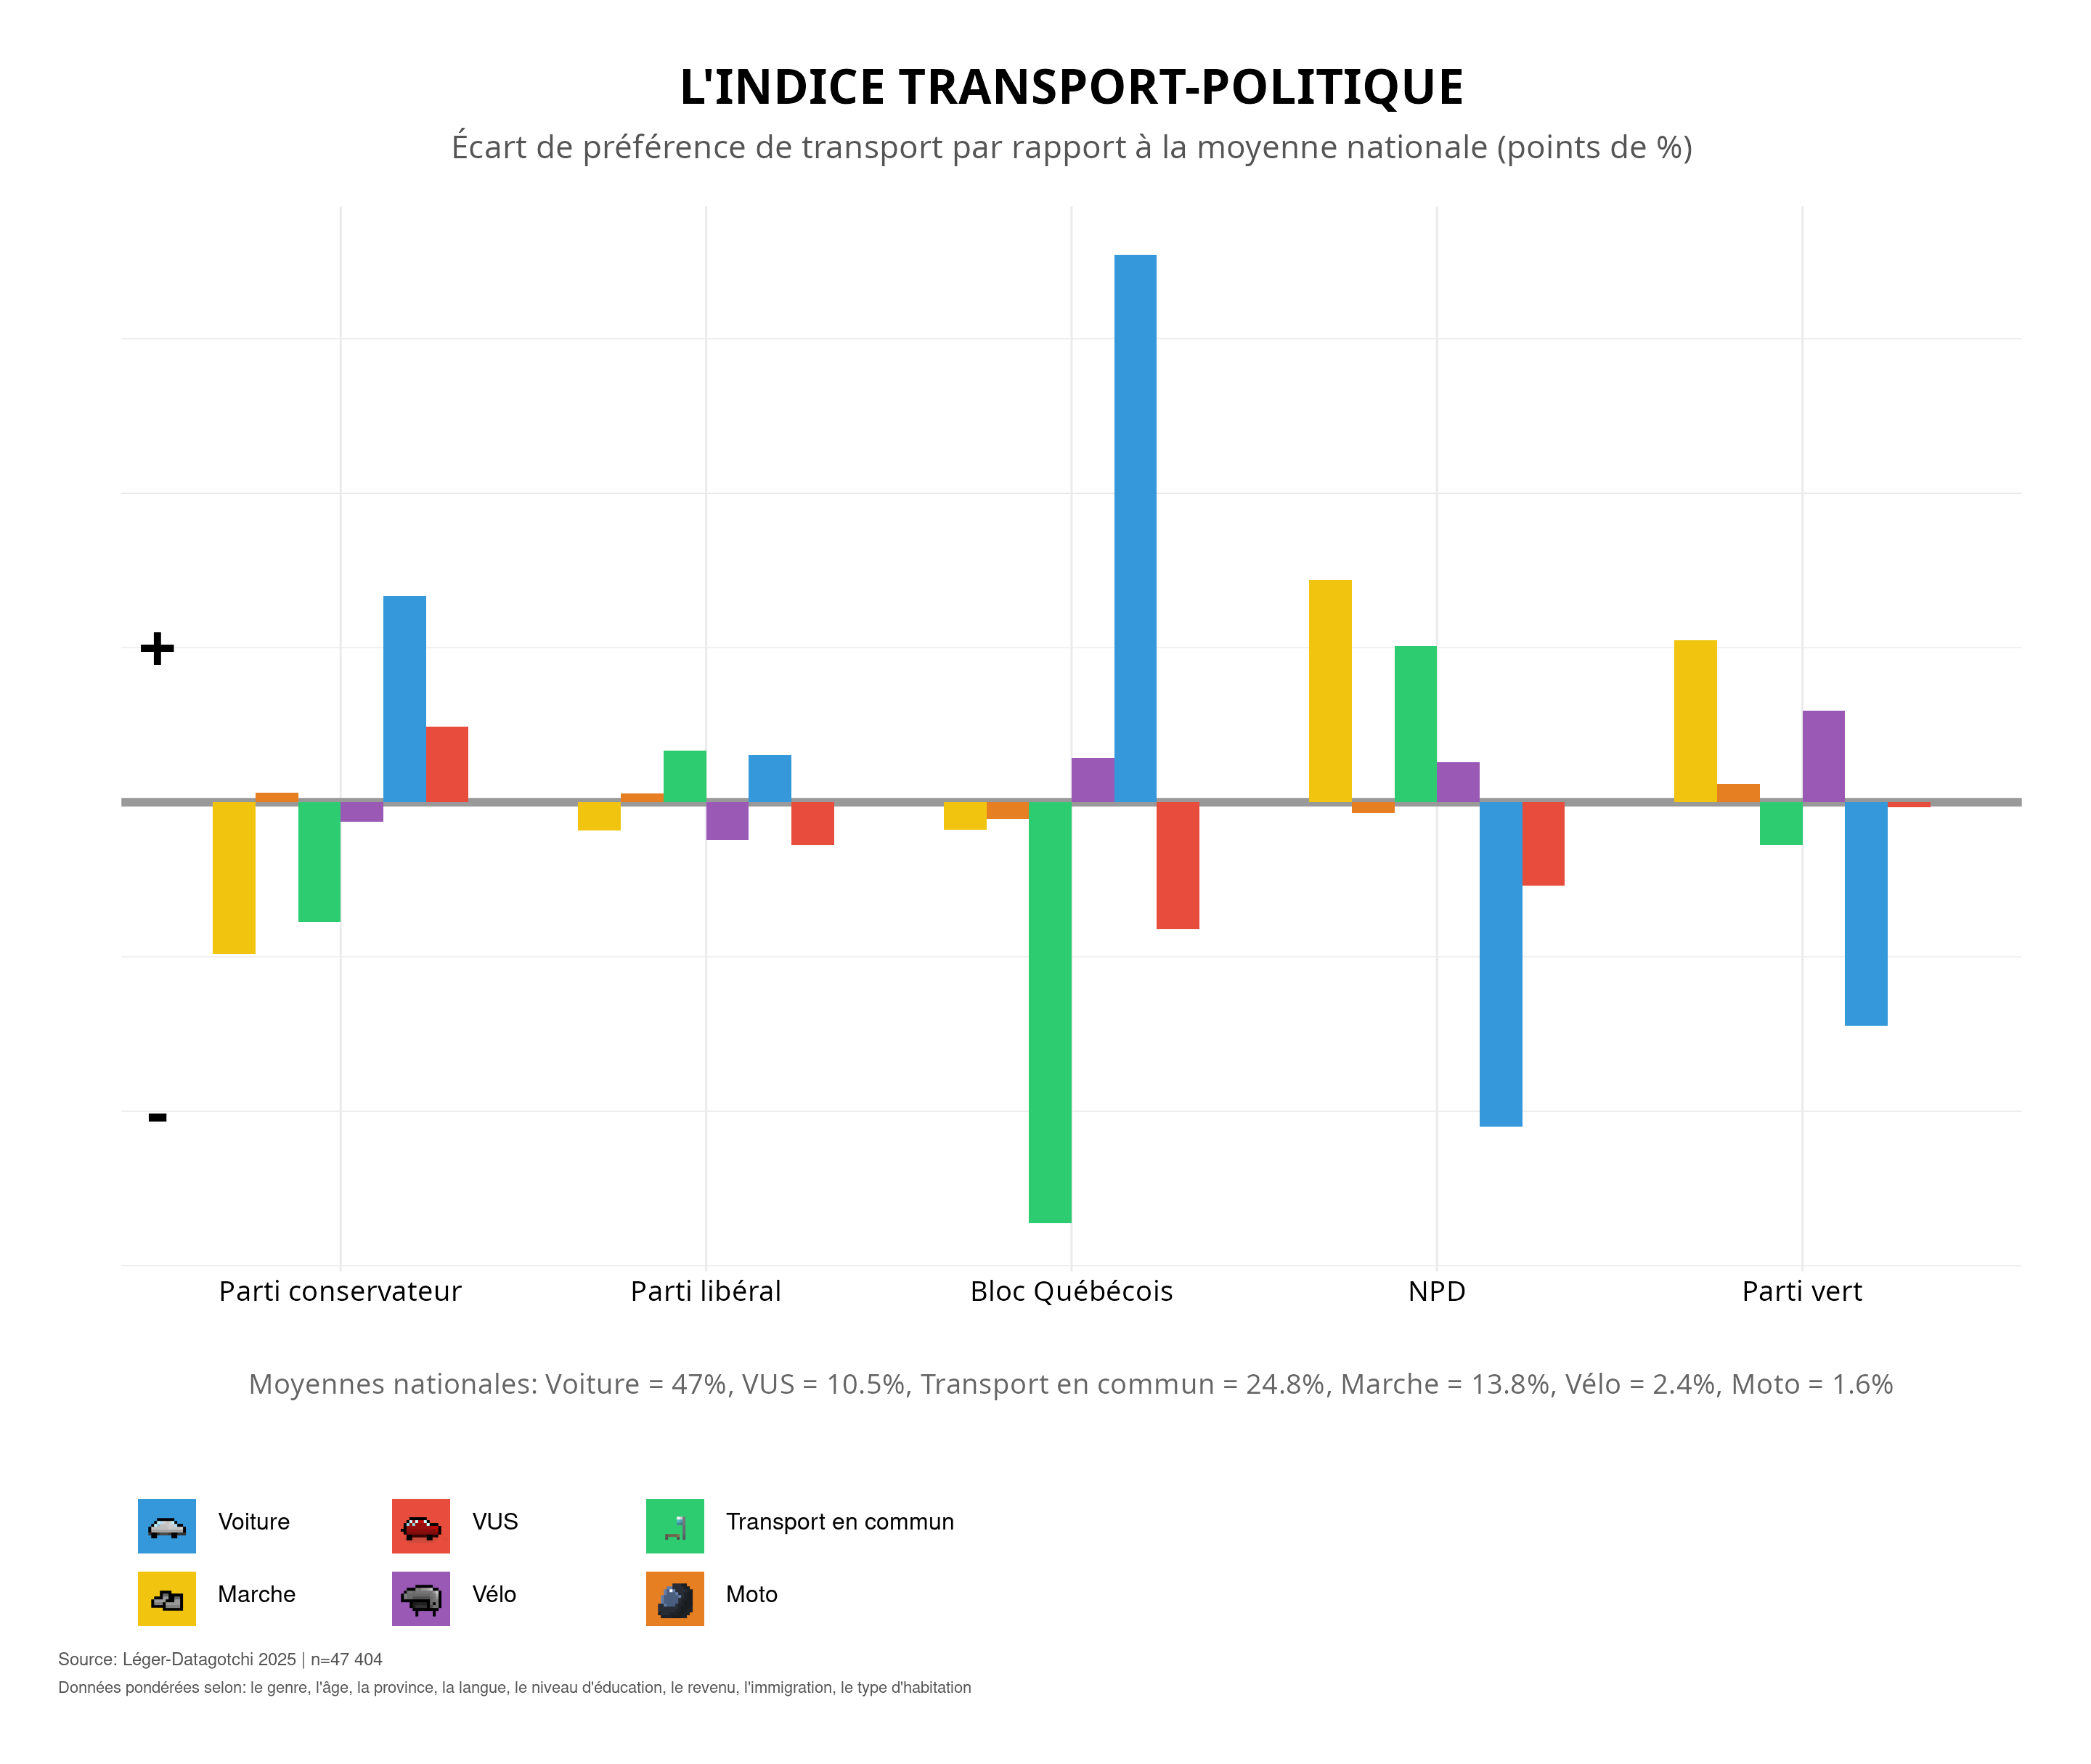
\includegraphics[width=0.9\textwidth,height=\textheight]{img/transport_graph.png}

}

\caption{Transport-Politics Index}

\end{figure}%%
\begin{figure}[H]

{\centering \includegraphics[width=0.9\textwidth,height=\textheight]{_SharedFolder_datagotchi_federal_2024/graph/analyses/transport/transport-vote-fr.png}

}

\caption{Transport-Politics (Detailed Version)}

\end{figure}%

The graph shows that BQ (Bloc Québécois) voters are the most
car-dependent (about 65\%), followed by the CPC (Conservative Party) at
about 53\% and the LPC (Liberal Party) at 47\%. The NDP and the Green
Party have higher rates of public transportation use (about 30\% and
23\% respectively) compared to other parties. For walking, the NDP
stands out with about 21\% of its voters, while Green Party voters are
the most numerous to use bicycles (about 5\%). Motorcycle use remains
marginal (less than 5\%) for all parties.




\end{document}
